Le viste definiscono la struttura delle pagine HTML e si occupano della visualizzazione delle informazioni richieste dall'utente e dell'invio delle HTTP Request al presenter. Le viste sono organizzate seguendo una classe base che definisce la struttura di una qualsiasi pagina HTML dell'applicazione. Ognuna delle pagine si riferisce a un determinato presenter.
\begin{itemize}
	\item \texttt{DeveloperView}: la vista dedicata allo sviluppatore che necessita di consultare i dati contenuti nella piattaforma; 
	\item \texttt{ProfileView}: la vista dedicata alla visualizzazione del profilo personale dell'utente e alle relative informazioni (ad esempio, la media degli esercizi per lo studente e il numero di esercizi assegnati per l'insegnante);
	\item \texttt{SearchView}: la vista dedicata alla visualizzazione delle pagine di ricerca della piattaforma;
	\item \texttt{ExerciseView}: la vista dedicata allo svolgimento e all'inserimento degli esercizi nella piattaforma.
\end{itemize}

\begin{figure}[h]
	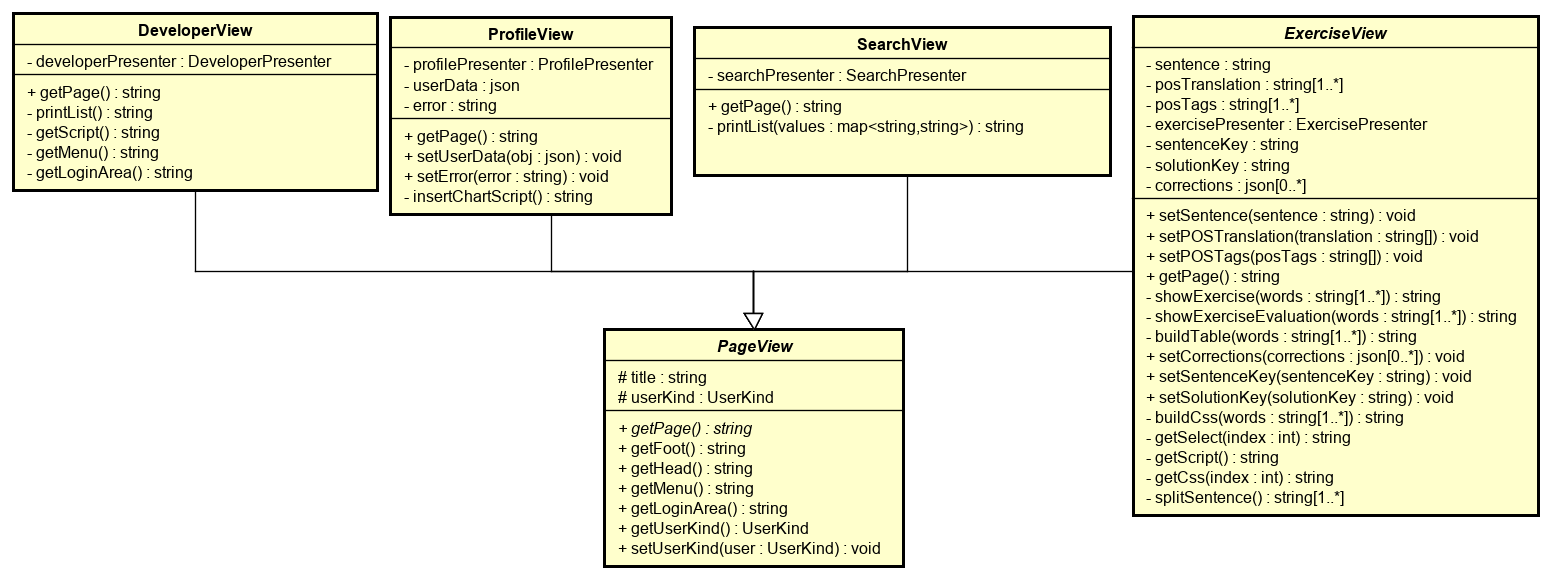
\includegraphics[scale=0.41]{images/View.png}
	\caption{Diagramma delle classi di View}
\end{figure}
